
%% paper.tex
%% for ISORC 2016
%% 2016/11/29
%% by Takuro Yamamoto

\documentclass[conference]{IEEEtran/IEEEtran}
% Some Computer Society conferences also require the compsoc mode option,
% but others use the standard conference format.
%
% If IEEEtran.cls has not been installed into the LaTeX system files,
% manually specify the path to it like:
% \documentclass[conference]{../sty/IEEEtran}

% Package List
%\usepackage[dvips]{graphics}
\usepackage[dvipdfmx]{graphicx}
\usepackage{amssymb}
\usepackage{float}
\usepackage{enumerate,cite,url}
\usepackage{listings,jlisting}
\lstset{%
    language={c},%
    basicstyle={\footnotesize\ttfamily},%
    identifierstyle={\footnotesize},%
    commentstyle={\footnotesize\itshape},%
    keywordstyle={\footnotesize},%\bfseries},%
    ndkeywordstyle={\footnotesize},%
    stringstyle={\footnotesize\it},
    frame={tb},
    breaklines=true,
    columns=[l]{fullflexible},%
    numbers=left,%
    xrightmargin=0zw,%
    xleftmargin=3zw,%
    numberstyle={\scriptsize},%
    stepnumber=1,
    numbersep=1zw,%
    lineskip=-0.5ex%
}

% *** Do not adjust lengths that control margins, column widths, etc. ***
% *** Do not use packages that alter fonts (such as pslatex).         ***
% There should be no need to do such things with IEEEtran.cls V1.6 and later.
% (Unless specifically asked to do so by the journal or conference you plan
% to submit to, of course. )


% correct bad hyphenation here
\hyphenation{op-tical net-works semi-conduc-tor}


\begin{document}
%
% paper title
% Titles are generally capitalized except for words such as a, an, and, as,
% at, but, by, for, in, nor, of, on, or, the, to and up, which are usually
% not capitalized unless they are the first or last word of the title.
% Linebreaks \\ can be used within to get better formatting as desired.
% Do not put math or special symbols in the title.
\title{TINET+TECS: Component-based TCP/IP Protocol Stack for Embedded Systems}


% author names and affiliations
% use a multiple column layout for up to three different
% affiliations
% \author{
% \IEEEauthorblockN{Takuro Yamamoto}
% \IEEEauthorblockA{Graduate School of Engineering Science\\Osaka University}
% \and
% \IEEEauthorblockN{Takuma Hara}
% \IEEEauthorblockA{Graduate School of Information Science\\Nagoya University}
% \and
% \IEEEauthorblockN{Takuya Ishikawa}
% \IEEEauthorblockA{Graduate School of Information Science\\Nagoya University}
% \and
% \IEEEauthorblockN{Hiroshi Oyama}
% \IEEEauthorblockA{OKUMA Corporation}
% \and
% \IEEEauthorblockN{Hiroaki Takada}
% \IEEEauthorblockA{Graduate School of Information Science\\Nagoya University}
% \and
% \IEEEauthorblockN{Takuya Azumi}
% \IEEEauthorblockA{Graduate School of Engineering Science\\Osaka University}
% }

% conference papers do not typically use \thanks and this command
% is locked out in conference mode. If really needed, such as for
% the acknowledgment of grants, issue a \IEEEoverridecommandlockouts
% after \documentclass

% for over three affiliations, or if they all won't fit within the width
% of the page, use this alternative format:
% 
\author{
\IEEEauthorblockN{
Takuro Yamamoto\IEEEauthorrefmark{1},
Takuma Hara\IEEEauthorrefmark{2},
Takuya Ishikawa\IEEEauthorrefmark{2}, 
Hiroshi Oyama\IEEEauthorrefmark{3},
Hiroaki Takada\IEEEauthorrefmark{2} and
Takuya Azumi\IEEEauthorrefmark{1}}
\IEEEauthorblockA{\IEEEauthorrefmark{1}Graduate School of Engineering Science, Osaka University}
\IEEEauthorblockA{\IEEEauthorrefmark{2}Graduate School of Information Science, Nagoya University}
\IEEEauthorblockA{\IEEEauthorrefmark{3}OKUMA Corporation}
}

% use for special paper notices
%\IEEEspecialpapernotice{(Invited Paper)}

% make the title area
\maketitle

% As a general rule, do not put math, special symbols or citations
% in the abstract
\begin{abstract}

Embedded systems are applied to Internet of Things (IoT), and the high productivity of embedded network software is required.
TINET is a TCP/IP protocol stack for embedded systems.
Although TINET is a compact TCP/IP protocol stack, it consists of many complex source codes.
Therefore, it is difficult to maintain, extend, and analysis the software.
To improve the scalability and configurability, this paper has proposed TINET+TECS, a component-based TCP/IP protocol stack for embedded systems: TINET componentized with TOPPERS embedded component system (TECS).
The component-based TINET provides software developers high productivity such as change of network buffer size and adding/removing TCP (or UDP) function.
We evaluate the component-based TINET compared with the original TINET.
We confirm that the overheads of execution time and memory consumption are low, and that the configurability is improved.

\end{abstract}

% no keywords

% For peer review papers, you can put extra information on the cover
% page as needed:
% \ifCLASSOPTIONpeerreview
% \begin{center} \bfseries EDICS Category: 3-BBND \end{center}
% \fi
%
% For peerreview papers, this IEEEtran command inserts a page break and
% creates the second title. It will be ignored for other modes.
\IEEEpeerreviewmaketitle

\section{Introduction}
\label{sec:Introduction}

Internet of Things (IoT) is an essential keyword for the next era \cite{par:IoTIndustries} \cite{par:IoTComputing}.
Various things, such as wearable devices, smart devices, and smart homes, connected to the Internet will enrich our lives.
Embedded systems are the elements constituting IoT, e.g., sensing data and controlling actuators.
It is not practical to implement the same TCP/IP protocol stack as a general computer because embedded systems have several restrictions such as low memory capacity.

TINET (Tomakomai InterNETworking) is a compact TCP/IP protocol stack for embedded systems \cite{url:TINET}.
TINET supports the ability such as minimum copy frequency and elimination of dynamic memory control.
TINET needs only small memory for its TCP/IP protocol stack; therefore it is suitable for embedded systems.
However, there are several issues that TINET consists of many complex source codes.
In other words, TINET is composed of many files and defines many macros.
This may take a lot of time for software developers to maintain, extend, and analysis the software.
Embedded network software is required for the high productivity and quality.

An approach to improve software productivity is component-based development, which is a design technique that can be applied to reusable software development for embedded systems \cite{par:Crnkovic}\cite{par:CBD}, such as TECS \cite{par:TECS} \cite{par:hr-tecs}, AUTOSAR \cite{url:AUTOSAR}, and SaveCCM \cite{par:SAVEapproach}.
Component-based systems are flexible to software extension and specification changes.
In addition, individual component diagrams enable the visualization of an entire system.

This paper proposes component-based TCP/IP protocol stack, i.e., TINET+TECS, to improve the configurability and scalability of software.
TECS (TOPPERS Embedded Component System) \cite{par:TECS} is utilized to componentize TINET, because TECS is a component system suitable for embedded systems.
TECS supports static configuration, which statically defines component behaviors and interconnections, thus TECS can optimize the overhead of componentization.

In addition, the proposed framework utilizes dynamic connection, a novel method of TECS, to switch component bindings dynamically.
A general TCP/IP protocol server dynamically processes the requested port i.e., HTTP (port: 80), HTTPS (prot: 443).
However, embedded systems can not dynamically generate components due to the strict memory restriction.
TINET+TECS statically generates components, and dynamically combines them.
Therefore, 

In the proposed framework, software application can be developed by not only TECS method but also existing method.
Software appication can be developed as a TECS component because TINET+TECS is a component-based framework using TECS.
Moreover, TECS supports an adapter to call functions of TECS components from non TECS codes.
The legacy codes such as an existing application can be supported in the proposed framework.

This paper evaluates the overheads of execution time and memory consumption and the amount of code line change for adding/removing the functionalities, which demonstrates TINET+TECS can improve the configurability with small overheads.

{\bf Contributions:} This paper provides the following contributions.

\begin{enumerate}

    \item {\bf Improve configurability}\mbox{}\\
        Since TINET+TECS is a component-based system, the software is flexible to change the configuration such as resizing network buffer, adding/removing TCP (or UDP) functions, and supporting both IPv4 and IPv6.
        In addition, a component diagram provides visualization of TINET, a complicated system.

    \item {\bf Dynamic connection method}\mbox{}\\
        Dynamically switching the binding of components, that is switching between a communication endpoint and reception point of TINET, realizes a TCP/IP protocol stack for embedded systems.
        
    \item {\bf Support legacy codes}\mbox{}\\
        TINET+TECS can be applied to an existing application because TECS supports the adapter to call TECS functions from C codes. 
    % \item {\bf Software visualization}

\end{enumerate}

{\bf Organization}: The remainder of this paper is organized as follows.
Section \ref{sec:System Model} introduces the system model and basic technologies, i.e., TINET and TECS.
Section \ref{sec:Design and Implementation} describes the design and implementation of the proposed framework.
Section \ref{sec:Evaluation and Demonstration} evaluates the proposed framework.
Related work is discussed in Section \ref{sec:Related Work}.
Conclusions and suggestions for future work are presented in Section \ref{sec:Conclusion}.


\section{System Model}
\label{sec:System Model}

This section describes system model, including the basic technologies such as TINET and TECS.
System model of the proposed framework is shown as Fig. \ref{fig:SystemModel}.
TINET+TECS is a component-based TCP/IP protocol stack, so TCP output task (tTCPOutput) and Ethernet input task (tEhternetInput) are implemented as TECS components.
CEP and REP (Section \ref{sec:TINET}), which are also implemented as TECS components, dynamically switch bindings by TECS method.
Moreover, TECS adapter supports the legacy codes such as an existing application.


\begin{figure}[t]
    \centering
    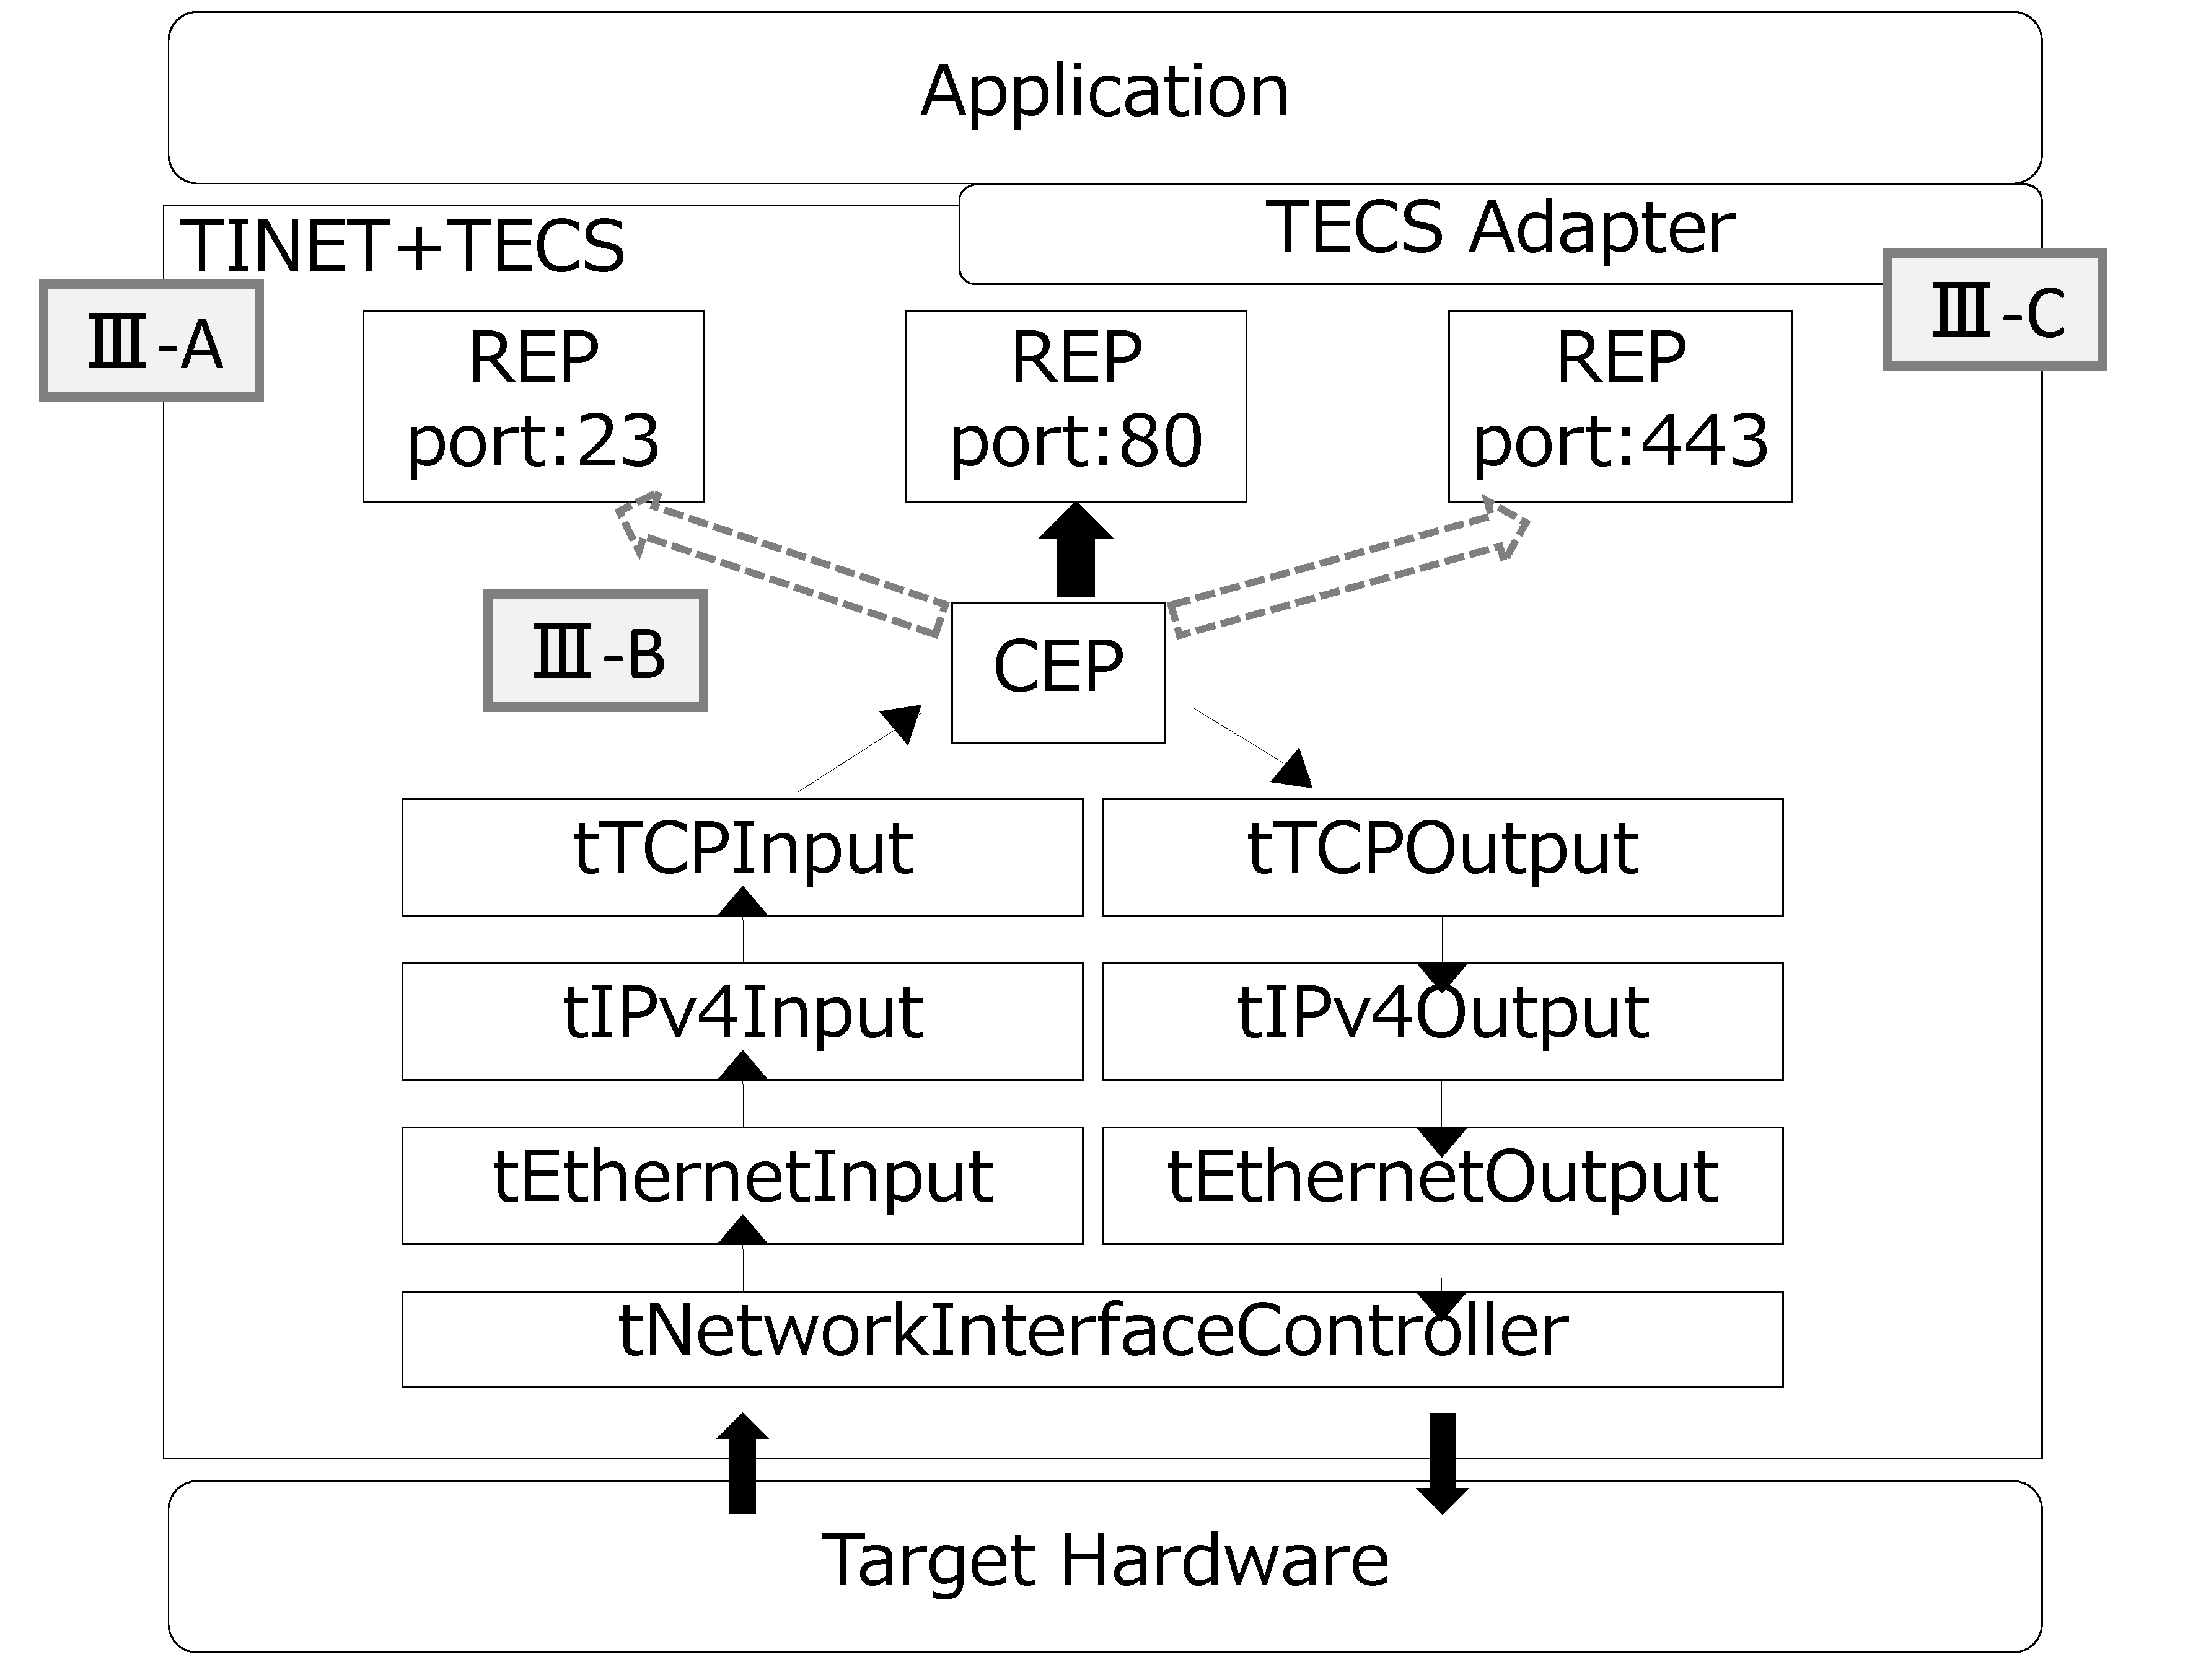
\includegraphics[width=7.0cm,clip]{figure/SystemModel.pdf}
    \caption{System model}
    \label{fig:SystemModel}
\end{figure}

\subsection{TINET}
\label{sec:TINET}

TINET is a compact TCP/IP protocol stack for embedded systems based on the ITRON\footnote{ITRON is a realtime operating system (RTOS) developed by TRON project.} TCP/IP API Specification \cite{url:ITRON_TCP/IP_API_Spec}, developed by TOPPERS (Toyohashi OPen Platform for Embedded Real-time Systems) Project \cite{url:TOPPERS}.
TINET has been released as open source.

To satisfy restrictions for embedded systems such as memory capacity, size, and power consumption, TINET supports following functions:

\begin{itemize}
    \item Minimum copy frequency
    \item Elimination of dynamic memory control
    \item Asynchronous interface
    \item Error detailed per API
\end{itemize}

\subsubsection{Overview}

TINET runs as middleware on TOPPERS/ASP3 \cite{par:ASP3} \cite{url:ASP3}, which is a realtime kernel based on $\mu$ITRON \cite{par:microITRON}.
TINET also supports other RTOSs such as TOPPERS/ASP and TOPPERS/JSP because TINET is compatible with TOPPERS RTOS.
Fig. \ref{fig:TINETHierarchyDiagram} shows the hierarchy diagram of TINET and TOPPERS/ASP3.
% TINET supports ITRON TCP/IP API such as {\it tcp\_snd\_buf}, {\it tcp\_rcv\_buf}, {\it udp\_snd\_buf}, and {\it udp\_rcv\_buf}.
Users transmit and receive the data using a Communication End Point (CEP) which is an interface like a socket.
In transmission process, headers are attached to the data body passed to the CEP at each protocol layer, and the data is transmitted from the network device.
In reception process, headers of the data body received in the network device are analyzed at each protocol layer, and the data is passed to the CEP.

A TCP reception point called Reception Point (REP) is prepared to wait for a connection request from the partner side.
An REP has an IP address ({\it myaddr}) and a port number ({\it myportno}) as attributes, and performs functions like {\it bind()} and {\it listen()}.

In TINET, the number of the data copy between each protocol layers is minimized.
A TCP/IP protocol stack for general computers has large overheads of execution time and memory consumption because the data is copied at each protocol layers.
To solve the problem, TINET does pass the pointer of the data buffer between each protocol layers, not perform data copy.

\begin{figure}[t]
    \centering
    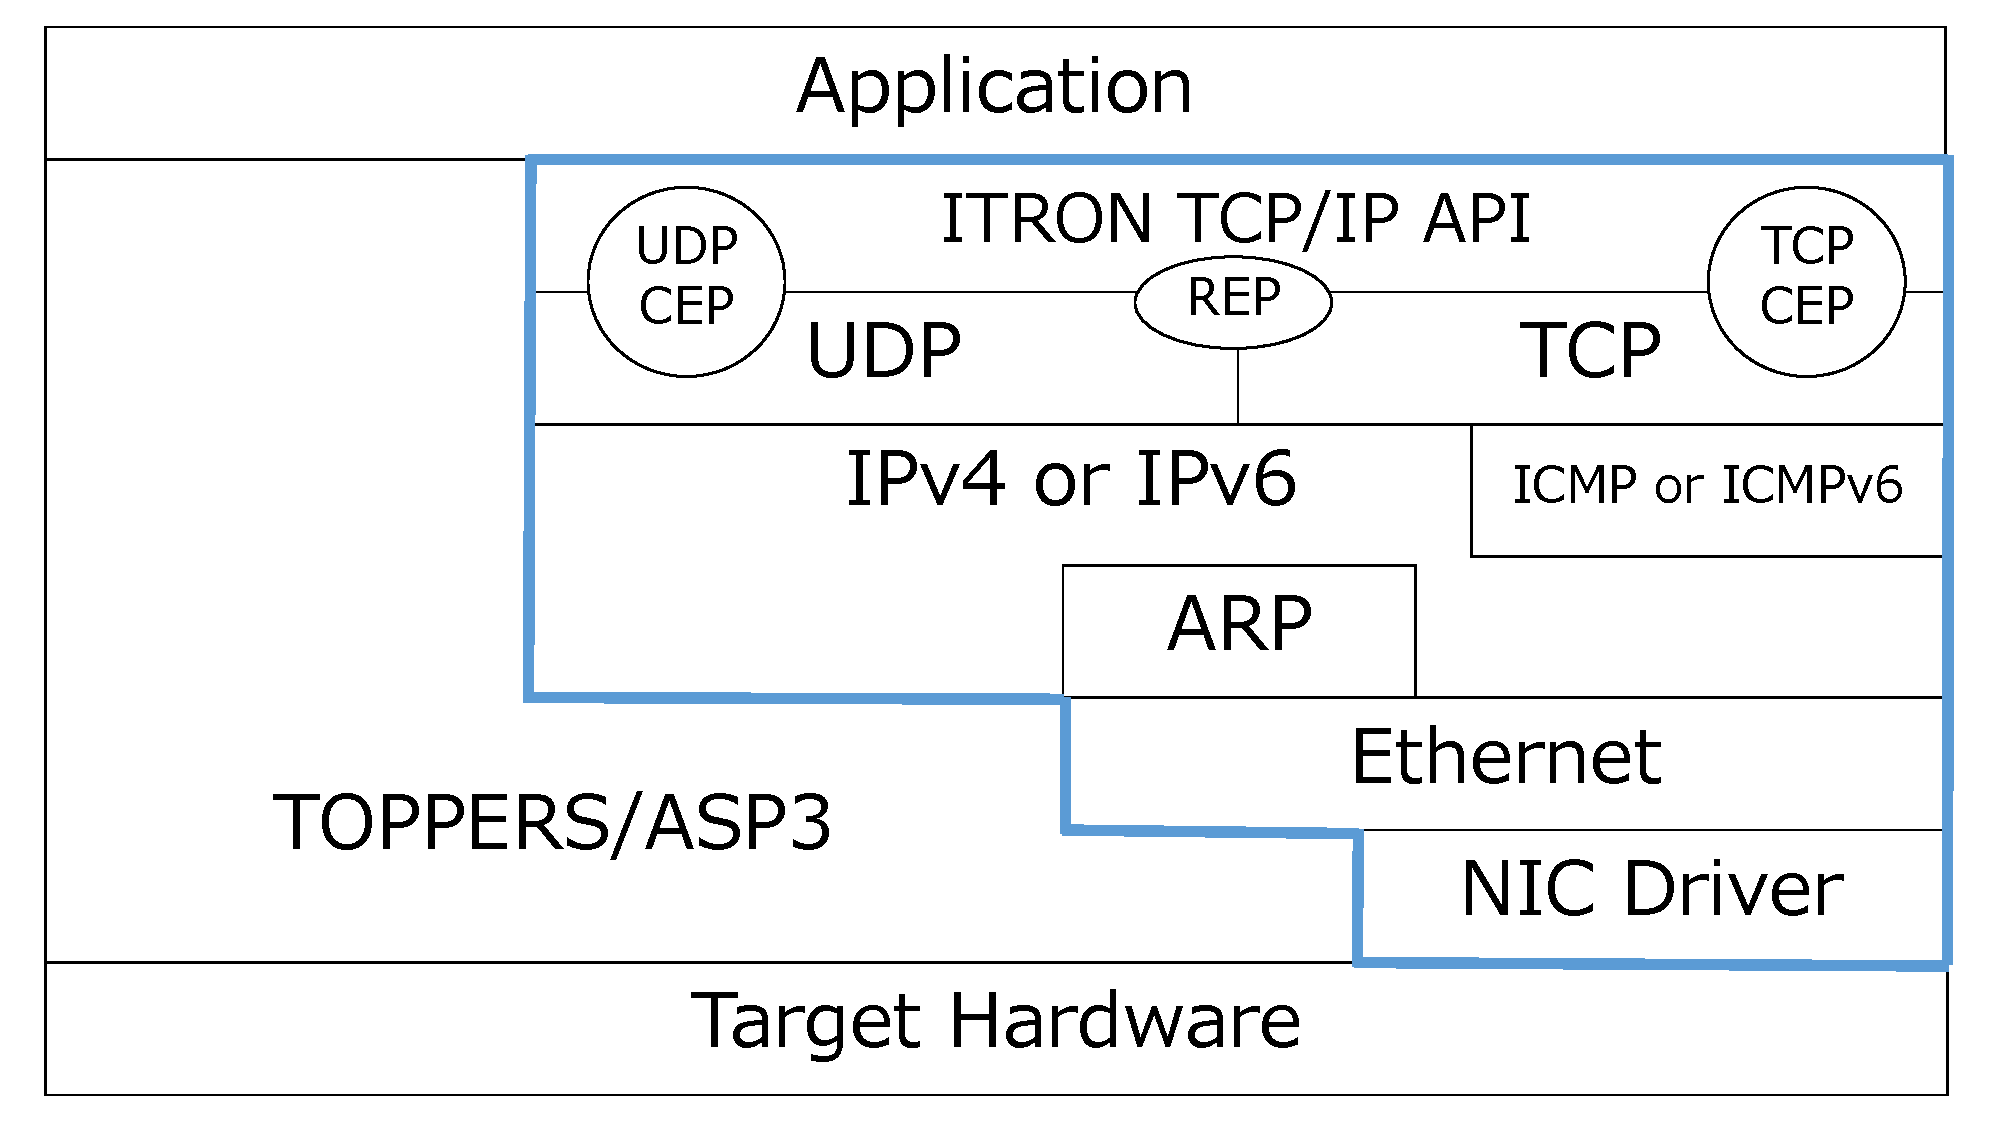
\includegraphics[width=7.0cm,clip]{figure/TINETHierarchyDiagram.pdf}
    \caption{Hierarchy diagram of TINET and TOPPERS/ASP3}
    \label{fig:TINETHierarchyDiagram}
\end{figure}

\subsection{TECS}
\label{sec:TECS}

TECS is a component system suitable for embedded systems.
TECS can increase productivity and reduce development costs owing to improved reusability of software components.
TECS also provides component diagrams, which help developers visualize the overall structure of a system.

In TECS, component deployment and composition are performed statically.
Consequently, connecting components does not incur significant overhead and memory requirements can be reduced.
TECS can be implemented in C, and demonstrates various feature such as source level portability and fine-grained components.

\begin{figure}[t]
    \centering
    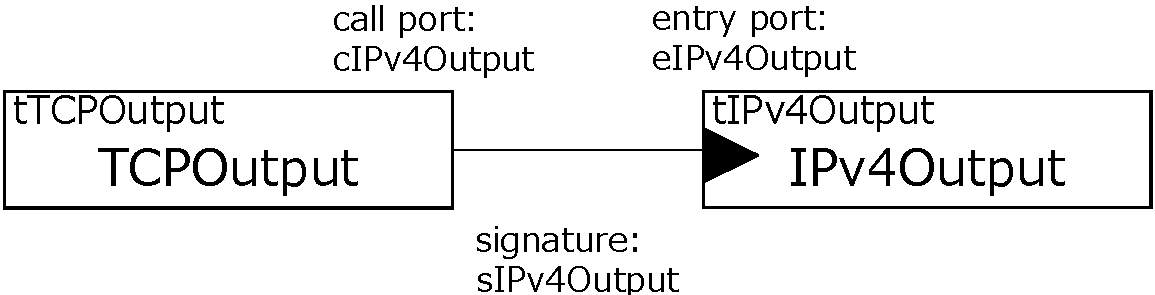
\includegraphics[width=7.0cm,clip]{figure/ComponentDiagram.pdf}
    \caption{Component Diagram}
    \label{fig:ComponentDiagram}
\end{figure}

\subsubsection{Component Model}

Fig. \ref{fig:ComponentDiagram} shows a component diagram.
A {\it cell}, which is an instance of a component in TECS, consists of {\it entry} ports, {\it call} ports, attributes and internal variables.
An {\it entry} port is an interface that provides functions to other {\it cell}s, and a {\it call} port is an interface that enables the use of other {\it cell}'s functions.
A {\it cell} has one or more {\it entry} ports and {\it call} ports.
{\it Cell} functions are implemented in C.

The type of {\it entry}/{\it call} port is defined by a {\it signature}, which is a set of functions.
A {\it signature} is the interface definition of a {\it cell}.
The {\it cell}'s  {\it call} port can be connected to the {\it entry} port of another {\it cell} by the same {\it signature}.
Note that {\it celltype} defines one or more {\it call}/{\it entry} ports, attributes, and internal variables of a {\it cell}.

\subsubsection{Component Description}

In TECS, components are described with component description language (CDL).
CDL can be divided into three categories: {\it signature}, {\it celltype}, and build description.
These components are described as follows.

\begin{description}
    \item[{\bf Signature Description}]\mbox{}\\
        The {\it signature} defines a {\it cell} interface.
        The {\it signature} name follows the keyword {\it signature} and takes the prefix ``s'', e.g., sIPv4Output (Fig. \ref{src:signature}).
        In TECS, to clarify the function of an interface, specifiers such as [in], [out], and [inout] are used, which represent input, output, and input/output respectively.
        [size\_is({\it len})] represents an array of size {\it len}.
\begin{figure}[t]
\centering
\begin{lstlisting}
signature sIPv4Output {
  T_IN4_ADDR getIPv4Address(void);
  ER         getOffset([inout]T_OFF_BUF *offset);
  ER         setHeader([inout,size_is(size)]
                        int8_t *outputp,
                        [in]int32_t size,
                        [in]T_IN4_ADDR dstaddr,
                        [in]T_IN4_ADDR srcaddr);
    /* Omit: other functions */
};
\end{lstlisting}
\caption{Signature description}
\label{src:signature}
\end{figure}
    \item[{\bf Celltype Description}]\mbox{}\\
        The {\it celltype} defines {\it entry} ports, {\it call} ports, attributes, and variables.
        A {\it celltype} name with the prefix ``t'' follows the keyword {\it celltype}, e.g., tIPv4Output (Fig. \ref{src:celltype}).
        To define {\it entry} ports, a {\it signature}, e.g., sIPv4Output, and an {\it entry} port name, e.g., eIPv4Output, follow the keyword {\it entry}.
        {\it Call} ports are defined similarly.
        Attributes and variables follow the keywords {\it attr} and {\it var}, respectively.
\begin{figure}[t]
\centering
\begin{lstlisting}
celltype tIPv4Output {
    /* Entry port */
    entry sIPv4Output eOutput;

    /* Call port */
    call sEthernetOutput cEthernetOutput;
    /* Omit: other call ports */

    attr {  /* Attribute */
        uint16_t fragInit = 0;
    };
    var {   /* Variable */
        uint16_t fragId = fragInit;
    };
};
\end{lstlisting}
\caption{Celltype description}
\label{src:celltype}
\end{figure}
    \item[{\bf Build Description}]\mbox{}\\
        The build description is used to instantiate and connect {\it cell}s.
        Fig. \ref{src:build} shows an example of a build description.
        A {\it celltype} name and {\it cell} name, e.g., tIPv4Output and IPv4Output, respectively, follow the keyword {\it cell}.
        A {\it call} port, {\it cell}'s name, and an {\it entry} port are described in that order to compose {\it cell}s,
        In Fig. \ref{src:build}, {\it entry} port eIPv4Output in {\it cell} IPv4Output is connected to {\it call} port cIPv4Output in {\it cell} TCPOutput.
        {\it C\_EXP} calls macros defined in C files.

\begin{figure}[t]
\centering
\begin{lstlisting}
cell tIPv4Output IPv4Output {
    /* Omit: other build description */
    
    fragInit = 0; /* Attribute */
};
cell tTCPOutput TCPOutput {
    cIPv4Output = IPv4Output.eOutput;
    /* Omit: other build description */
};
\end{lstlisting}
\caption{Build description}
\label{src:build}
\end{figure}

\end{description}

\section{Design and Implementation}
\label{sec:Design and Implementation}

This section describes design and implementation of the proposed framework, TINET+TECS.
The proposed framework is component-based TCP/IP protocol stack for embedded systems, i.e., componentized TINET using TECS.
In addition, A TECS novel functionality, dynamic connection method, and TECS adapter to support legacy codes are described with the use case of the proposed framework.

\subsection{TINET+TECS}
TINET+TECS, the proposed componentized TCP/IP protocol stack, consists of some TECS components.
This section describes the components of TINET+TECS framework with component diagrams.
% In addition, TECS functionalities applied to the proposed system such as {\it send}/{\it receive} specifier and adapter are explained.

\subsubsection{Components of protocol stack}

The components of protocol stack for TINET+TECS is shown as Fig. \ref{fig:ComponentProtocolStack}.
Note that some small particle components such as a kernel object, dataqueques, and semaphores are omitted to simplify the component diagram.
In TINET+TECS, the components are divided for each protocol, and the functionalities such as input function and output function are defined as each a component.
Therefore, software visibility is improving because of small grain components.

\begin{figure}[t]
    \centering
    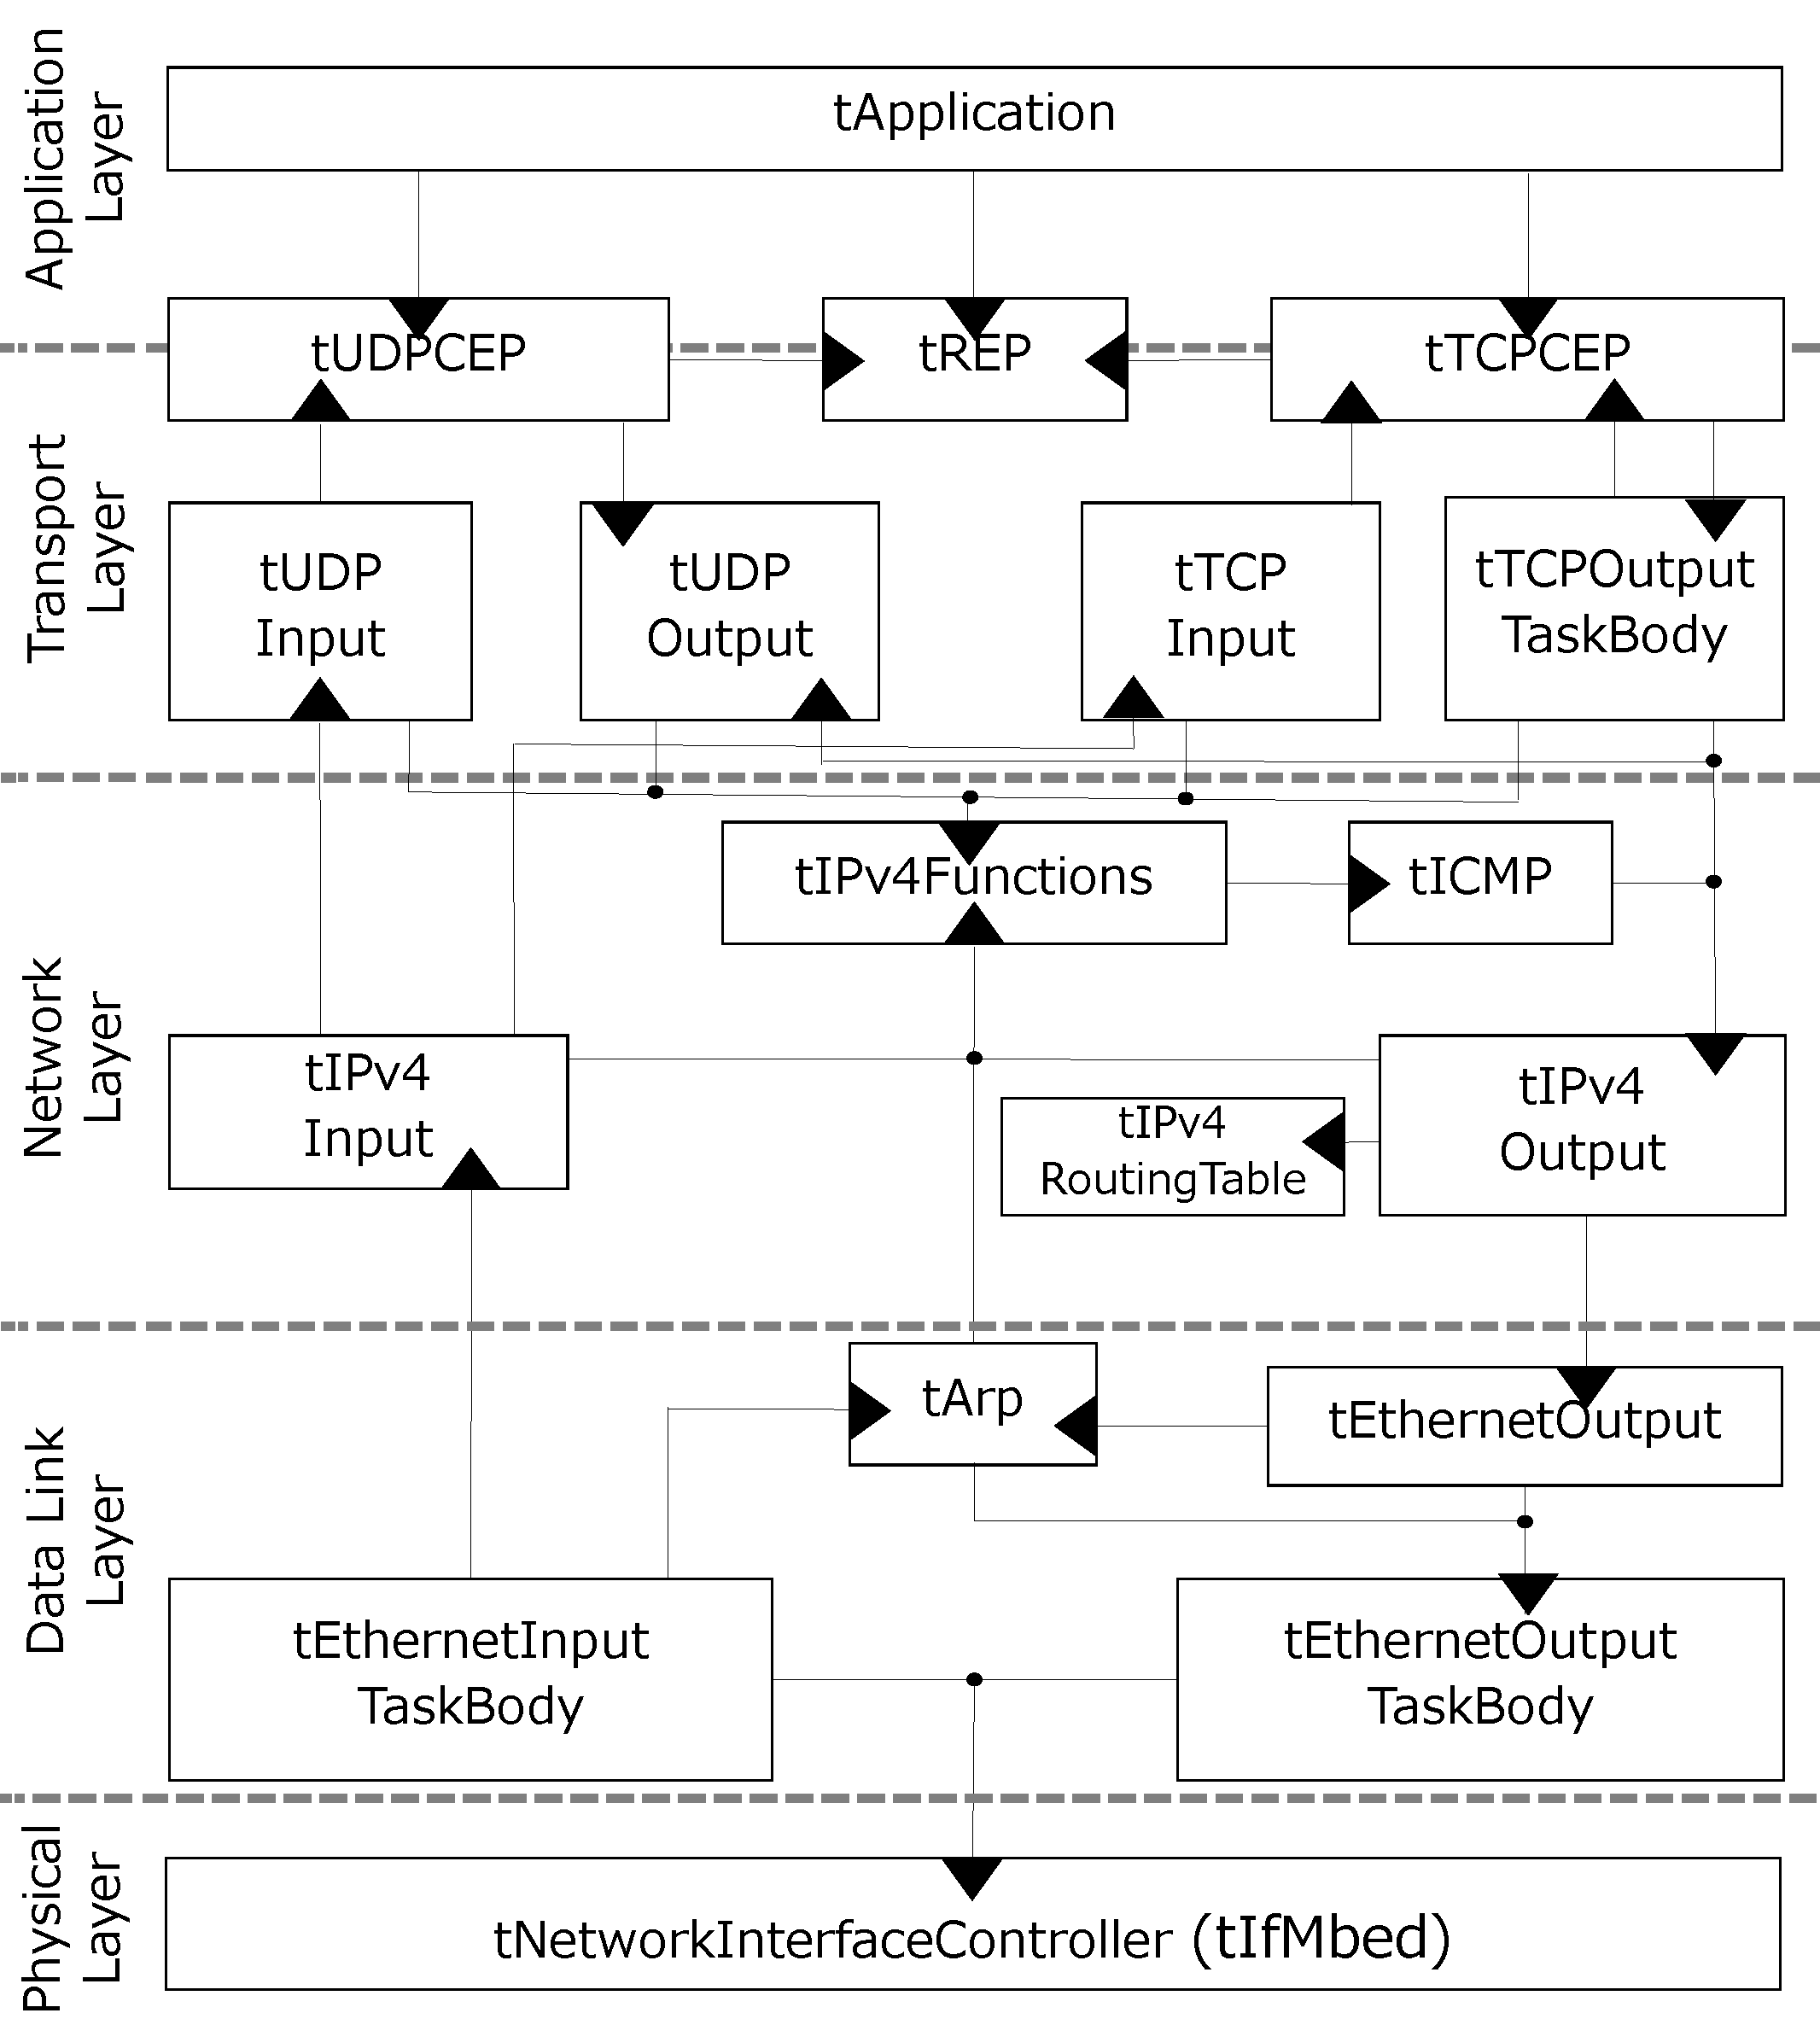
\includegraphics[width=7.0cm,clip]{figure/ComponentProtocolStack.pdf}
    \caption{Component diagram of protocol stack}
    \label{fig:ComponentProtocolStack}
\end{figure}

The components of each protocol are described below.\\

{\bf Application layer:}
An application in TINET+TECS is implemented as a component such as tApplication.
Software with TINET uses ITRON TCP/IP API such as {\it tcp\_snd\_buf} and {\it tcp\_rcv\_buf}.
In TINET+TECS, the application component calls TECS functions such as {\it cTCPAPI\_sendBuffer} and {\it cTCPAPI\_receiveBuffer}.
Moreover, TINET+TECS supporting a TECS adapter (\ref{sec:TECS Adapter}), an exiting application with TINET can run on TINET+TECS framework without transporting.
Therefore, software can be developed either with exiting methods or as a TECS component.

{\bf Transport layer:}
tTCPCEP (tUDPCEP) is a CEP compornent for TCP (UDP), and tREP is a REP component.
For example, a server program supporting multiple clients can be developed by preparing the multiple tTCPCEP components.
tTCPInput (tUDPInput) and tTCPOutput (tUDPOutput) are components performing the receiving and sending processing respectively in the transport layer.

{\bf Network layer:}
tIPv4Input and tIPv4Output are components performing the receiving and sending processing respectively in the network layer.
tIPv4Functions component performs some functions such as checksum, tICMP component is for the ICMP protocol, and tIPv4RoutingTable component operates a routing table.

{\bf Data link layer:}
tEthernetInputTaskBody and tEthernetOutputTaskBody (tEthernetOutput) are components performing the receiving and sending processing respectively in the data link layer.
tArp component is for the ARP protocol.

{\bf Physical layer:}
tNetworkInterfaceContoroller component implements a network device driver.
Software can run on other devices by replacing the component because only the component depends on the target device.\\

To utilize the protocol stack as same as the original TINET, communication object components such as tTCPCEP, tUDPCEP, and tREP are defined as an interface between TINET+TECS and an application.
The communication object component is a component corresponding to a CEP or REP of the original TINET.
An application developers can utilize the TINET+TECS functionalities by generating and combining as many components as necessary.

The protocol stack of TINET+TECS supports coexistence of multiple protocols.
By developing the IPv6 and Point-to-Point Protocol (PPP) components, TINET+TECS can make IPv4 and IPv6 coexist and support PPP without a modification of component implementation.

\subsubsection{Memory allocator component} 

The original TINET eliminates dynamic memory control to meet the sever memory restriction of embedded systems.
A memory area for sending/receiving data in the protocol stack is allocated and released within an predetermined area.
Memory allocator component performs the elimination of dynamic memory control in TINET+TECS.
The component provides a requested memory area from the memory area statically allocated.

The memory allocator component connects to as many tFixedSizeMemoryPool as needed, shown as Fig. \ref{fig:tMemoryAllocator}.
tFixedSizeMemoryPool is a componentized kernel object of TOPPERS/ASP3 to alloc and release a memory area of the requested size. 
tFixedSizeMemoryPool components with various sizes are prepared, and an appropriate memory area can be allocated according to the used data size.
On the other hands, all components which need allocate and deallocate memory connect to the memory allocator component, e.g., tTCPInput and tEthernetOutput.

In addition, TINET+TECS utilizes {\it send/receive} specifier of TECS to minimize the memory copy frequency, which is a functionality supported by TINET.

\begin{figure}[t]
    \centering
    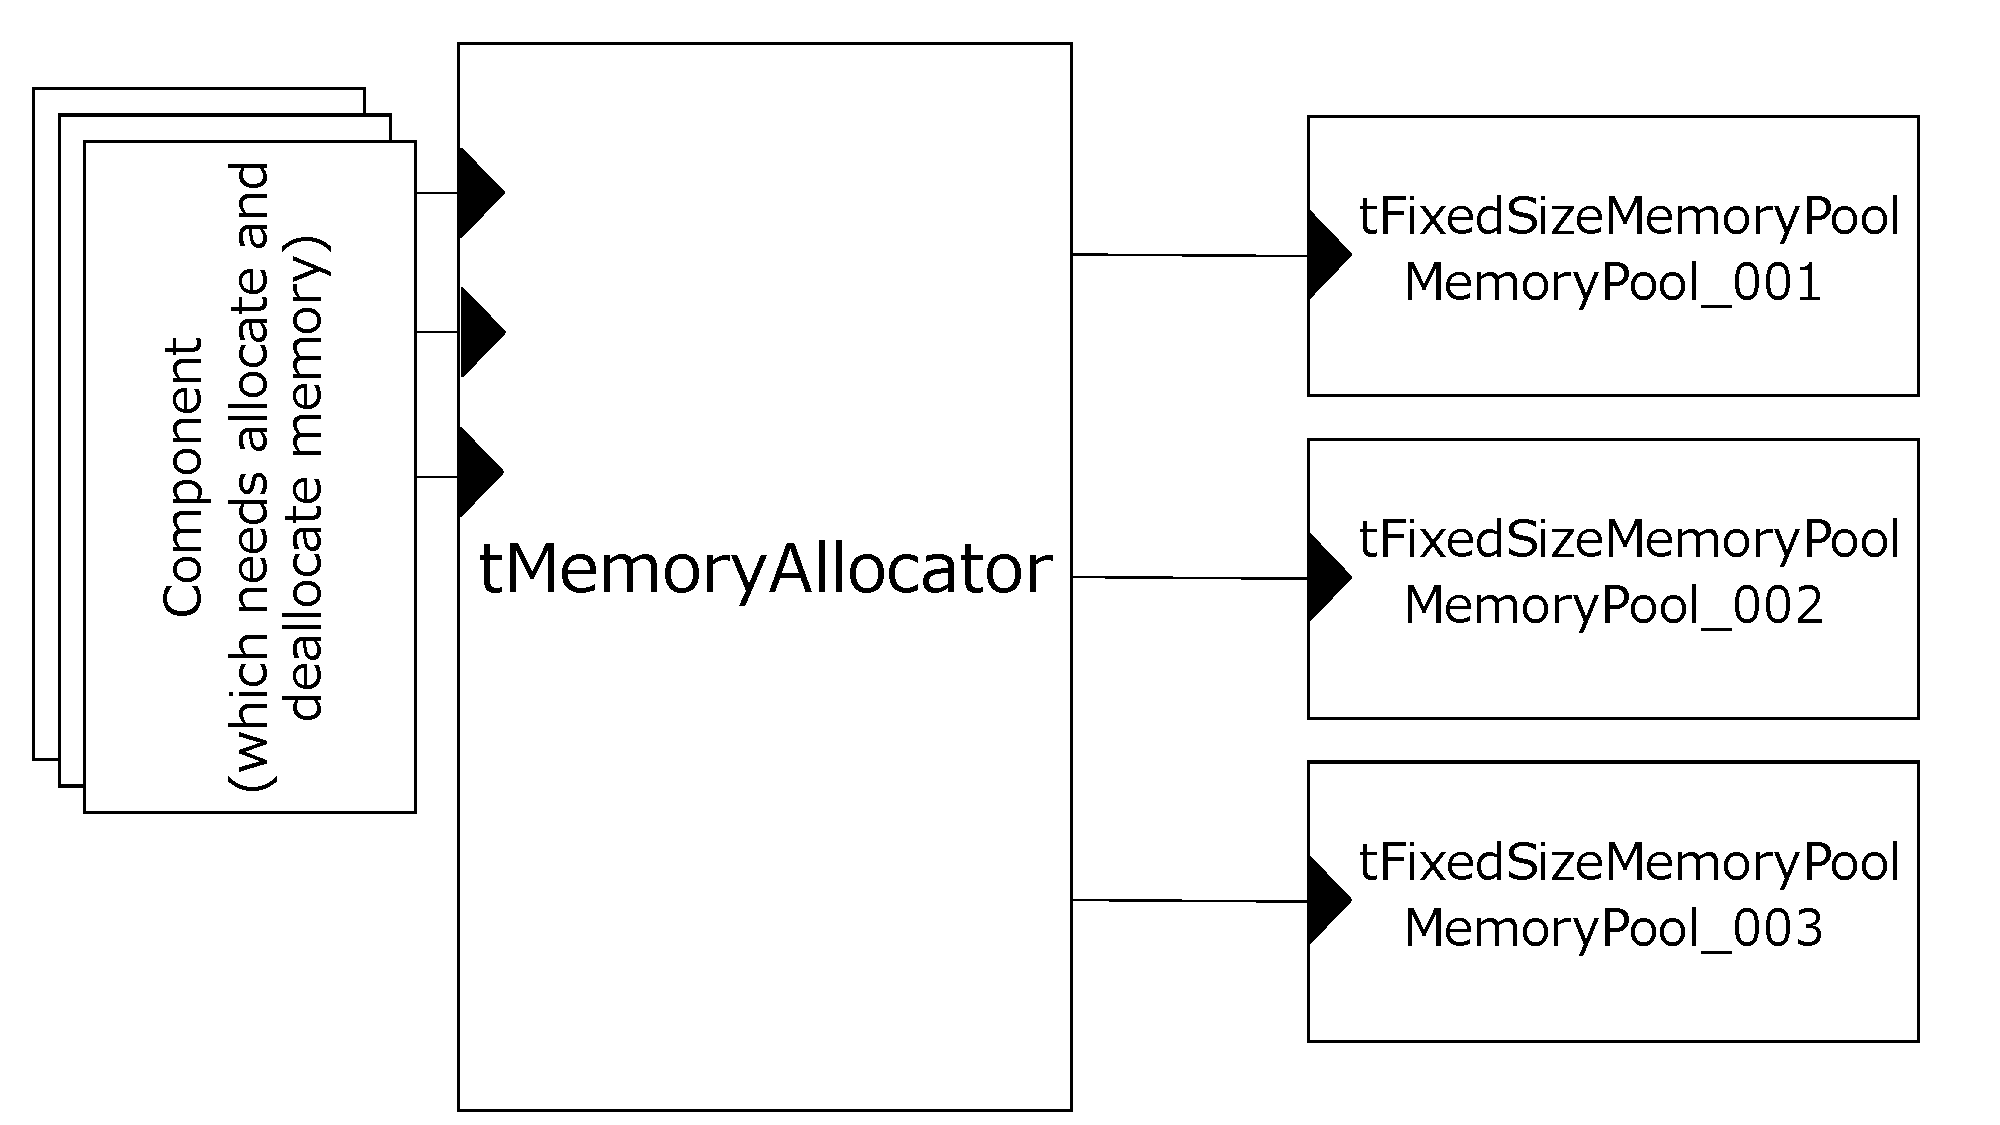
\includegraphics[width=7.0cm,clip]{figure/tMemoryAllocator.pdf}
    \caption{Component diagram of tMemoryAllocator}
    \label{fig:tMemoryAllocator}
\end{figure}

\begin{figure}[t]
    \centering
    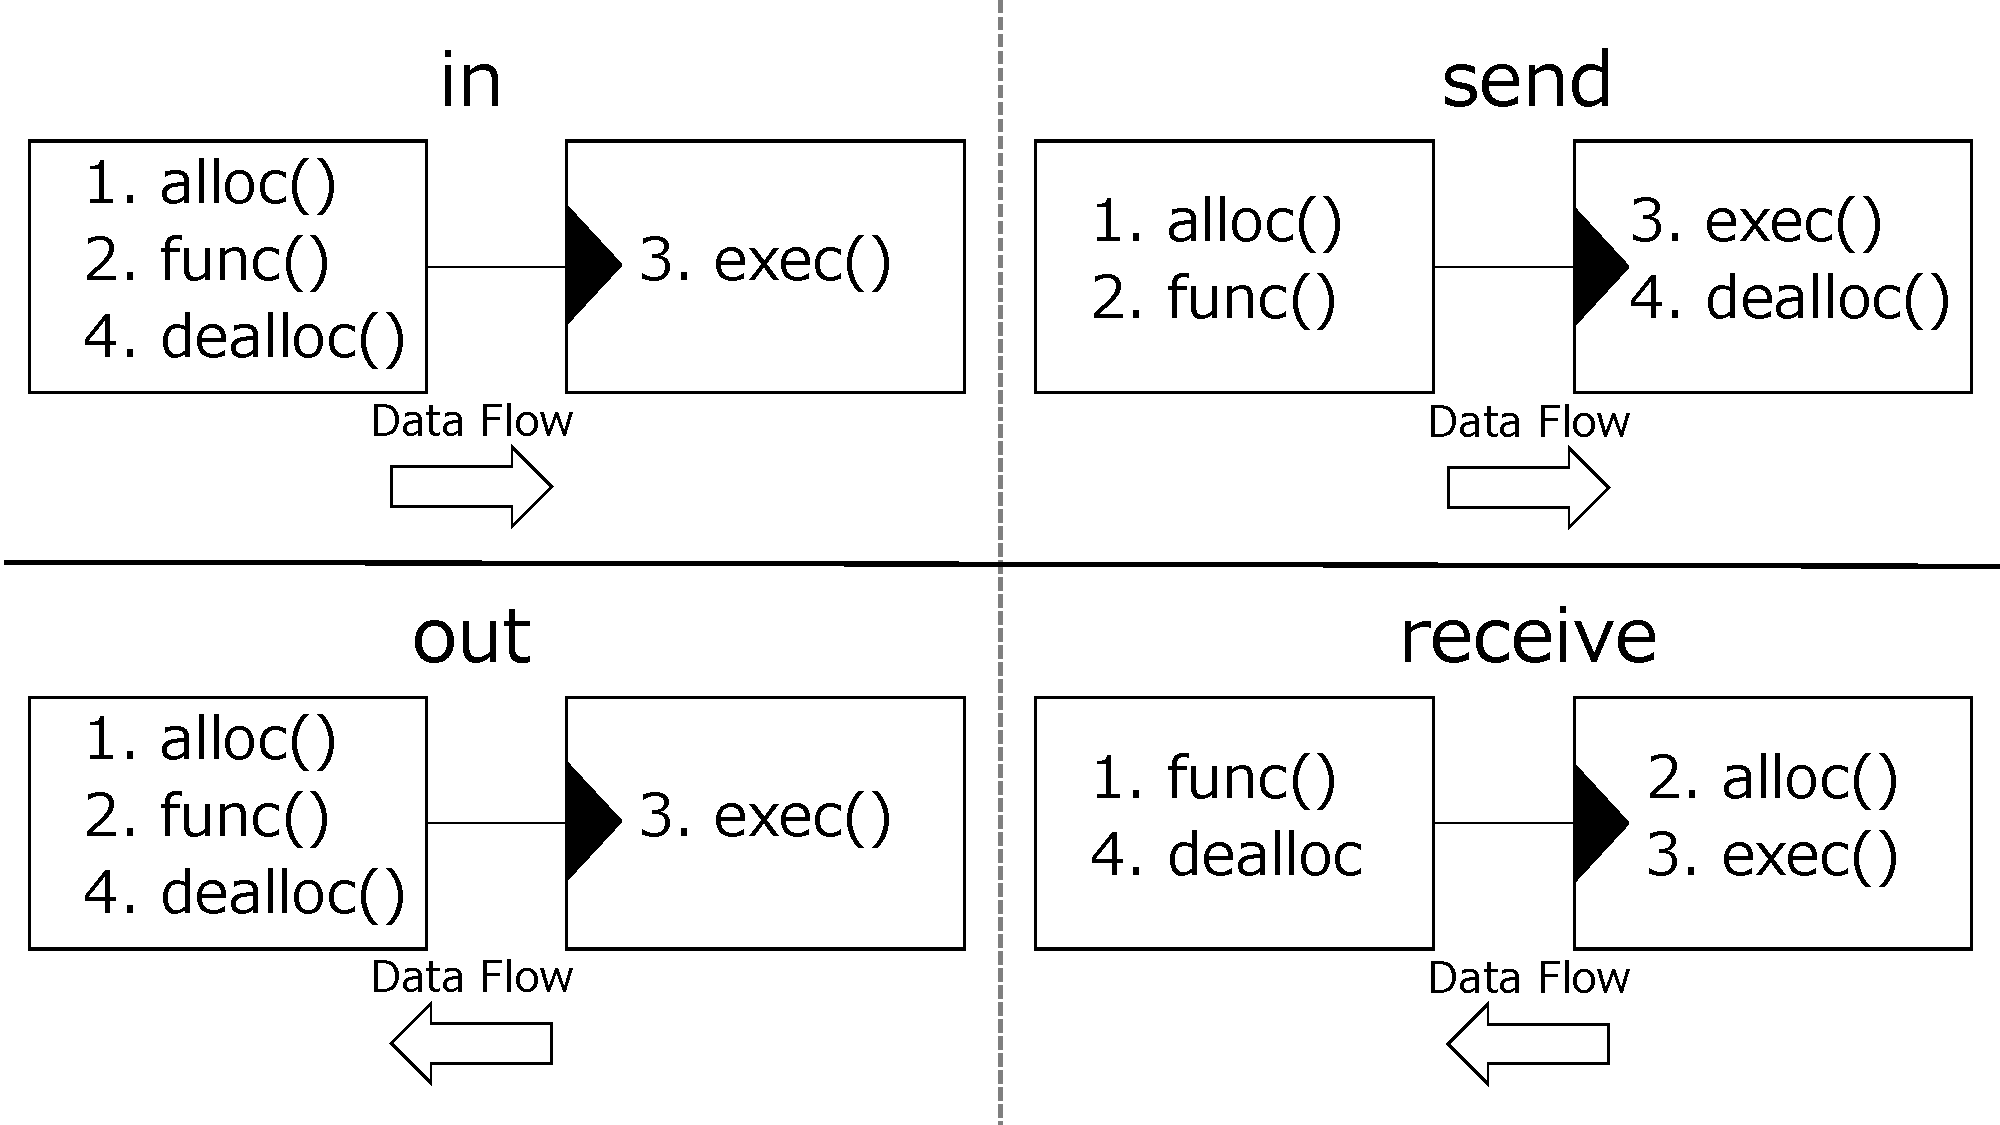
\includegraphics[width=7.0cm,clip]{figure/SendReceive.pdf}
    \caption{Differences between in/out and send/receive}
    \label{fig:SendReceive}
\end{figure}

{\bf send/receive specifier:}
TECS supports {\it send}/{\it receive} specifiers, which are interface specifiers \cite{par:RPC}.
TINET+TECS uses {\it send} and {\it receive} specifiers instead of {\it in} and {\it out} to reduce the number of copies.

{\it in} is a specifier for input arguments.
A callee side uses the memory of arguments with {\it in} during executing the callee function.
When the processing returns to the caller side, the caller can reuse and deallocate the memory.

{\it send} is also a specifier for transferring data to a callee from a caller such as {\it in}.
The difference between {\it in} and {\it send} is whether to deallocate the data memory in a caller or callee, shown as Fig. \ref{fig:SendReceive}.
In case of {\it in} specifier, both allocating and deallocating the data memory are performed in the caller.
On the other hand, in case of {\it send}, the caller allocates the data memory and the callee deallocates it.

{\it out} is a specifier for output arguments.
A callee writes data in the memory allocated by a caller, and the caller receives the data.

{\it receive} is also a specifier for a caller receiving data from a callee such as {\it out}.
The difference between {\it out} and {\it receive} is whether to allocate the data memory in a caller or callee, shown as Fig. \ref{fig:SendReceive}.
While, in case of {\it out}, a callee writes data in the memory allocated by a caller, in case of {\it receive}, the callee allocates the data memory.
Deallocating the memory is performed in the caller in both cases.


\begin{figure}[t]
\centering
\begin{lstlisting}
signature sNicDriver {
  void start(
    [send(sNetworkAlloc),size_is(size)]
        int8_t *outputp,
    [in]int32_t size,
    [in]uint8_t align);
  void read(
    [receive(sNetworkAlloc),size_is(*size)]
        int8_t **inputp,
    [out]int32_t *size,
    [in]uint8_t align);
    /* Omit: other functions */
};
\end{lstlisting}
\caption{An example of send and receive}
\label{src:SendReceive}
\end{figure}

\subsubsection{Network timer component}


\subsection{Dynamic Connection of TECS}
\label{sec:DynamicConnection}

\begin{figure}[t]
    \centering
    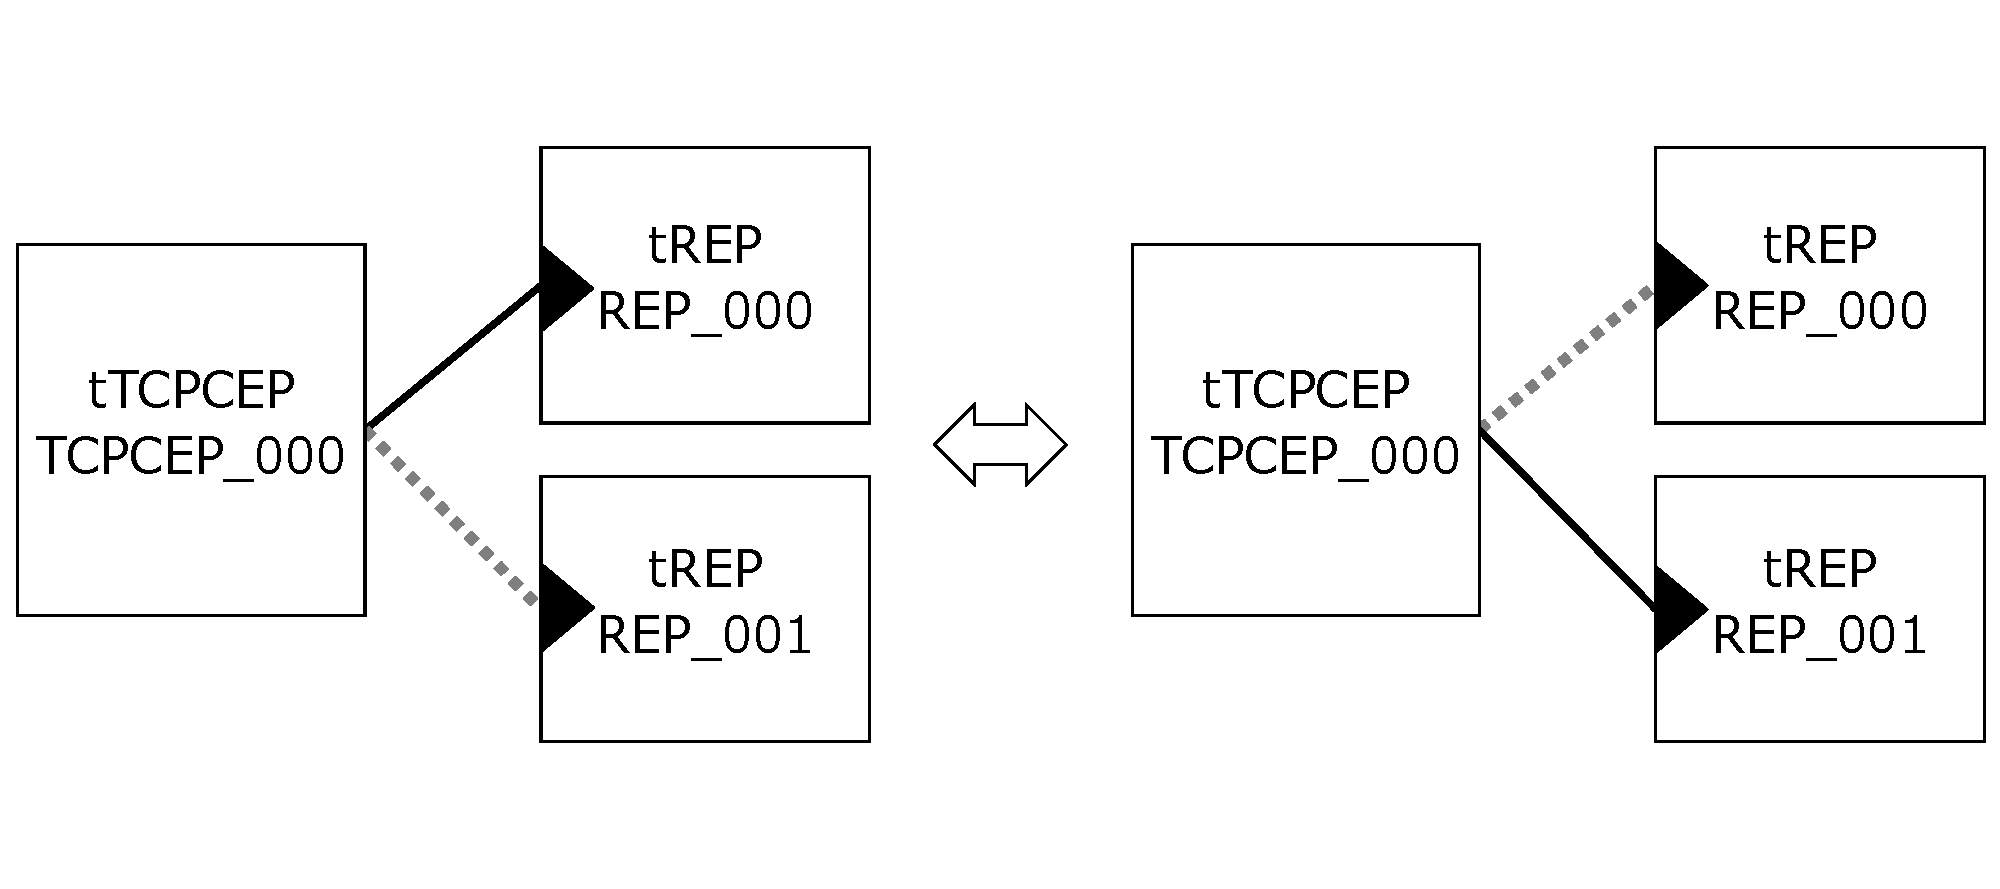
\includegraphics[width=7.0cm,clip]{figure/DynamicConnection.pdf}
    \caption{Dynamic connection}
    \label{fig:DynamicConnection}
\end{figure}

TECS supports dynamic connection method as a novel functionality.
Dynamic connection is a method to switch the binding of components at runtime as shown in Fig. \ref{fig:DynamicConnection}.
Note that all components are statically generated in TECS.
TECS can optimize the overhead of componentization because components are statically configured.
Dynamically generating the components causes a lot of memory consumption, which is a serious propoblem for embedded systems with strict memory constraint.
The proposed framework realizes the componentization of TINET while satisfying the memory constraint, because components statically generate and dynamically connect in TECS.

TINET+TECS utilizes the dynamic connection to swith between CEP and REP components as shown in Fig. \ref{fig:DynamicConnectionUseCase}.
In a server application, CEP is associated with REP in the state waiting for connection request from clients\footnote{ITRON TCP/IP API Specification \cite{url:ITRON_TCP/IP_API_Spec}\\tcp\_acp\_cep(ID cepid, ID repid, T\_IPV4EP *p\_dstaddr, TMO tmout)}.
For example, when processing with HTTP protocol, CEP passively opens with REP of port number 80.

\begin{figure}[t]
    \centering
    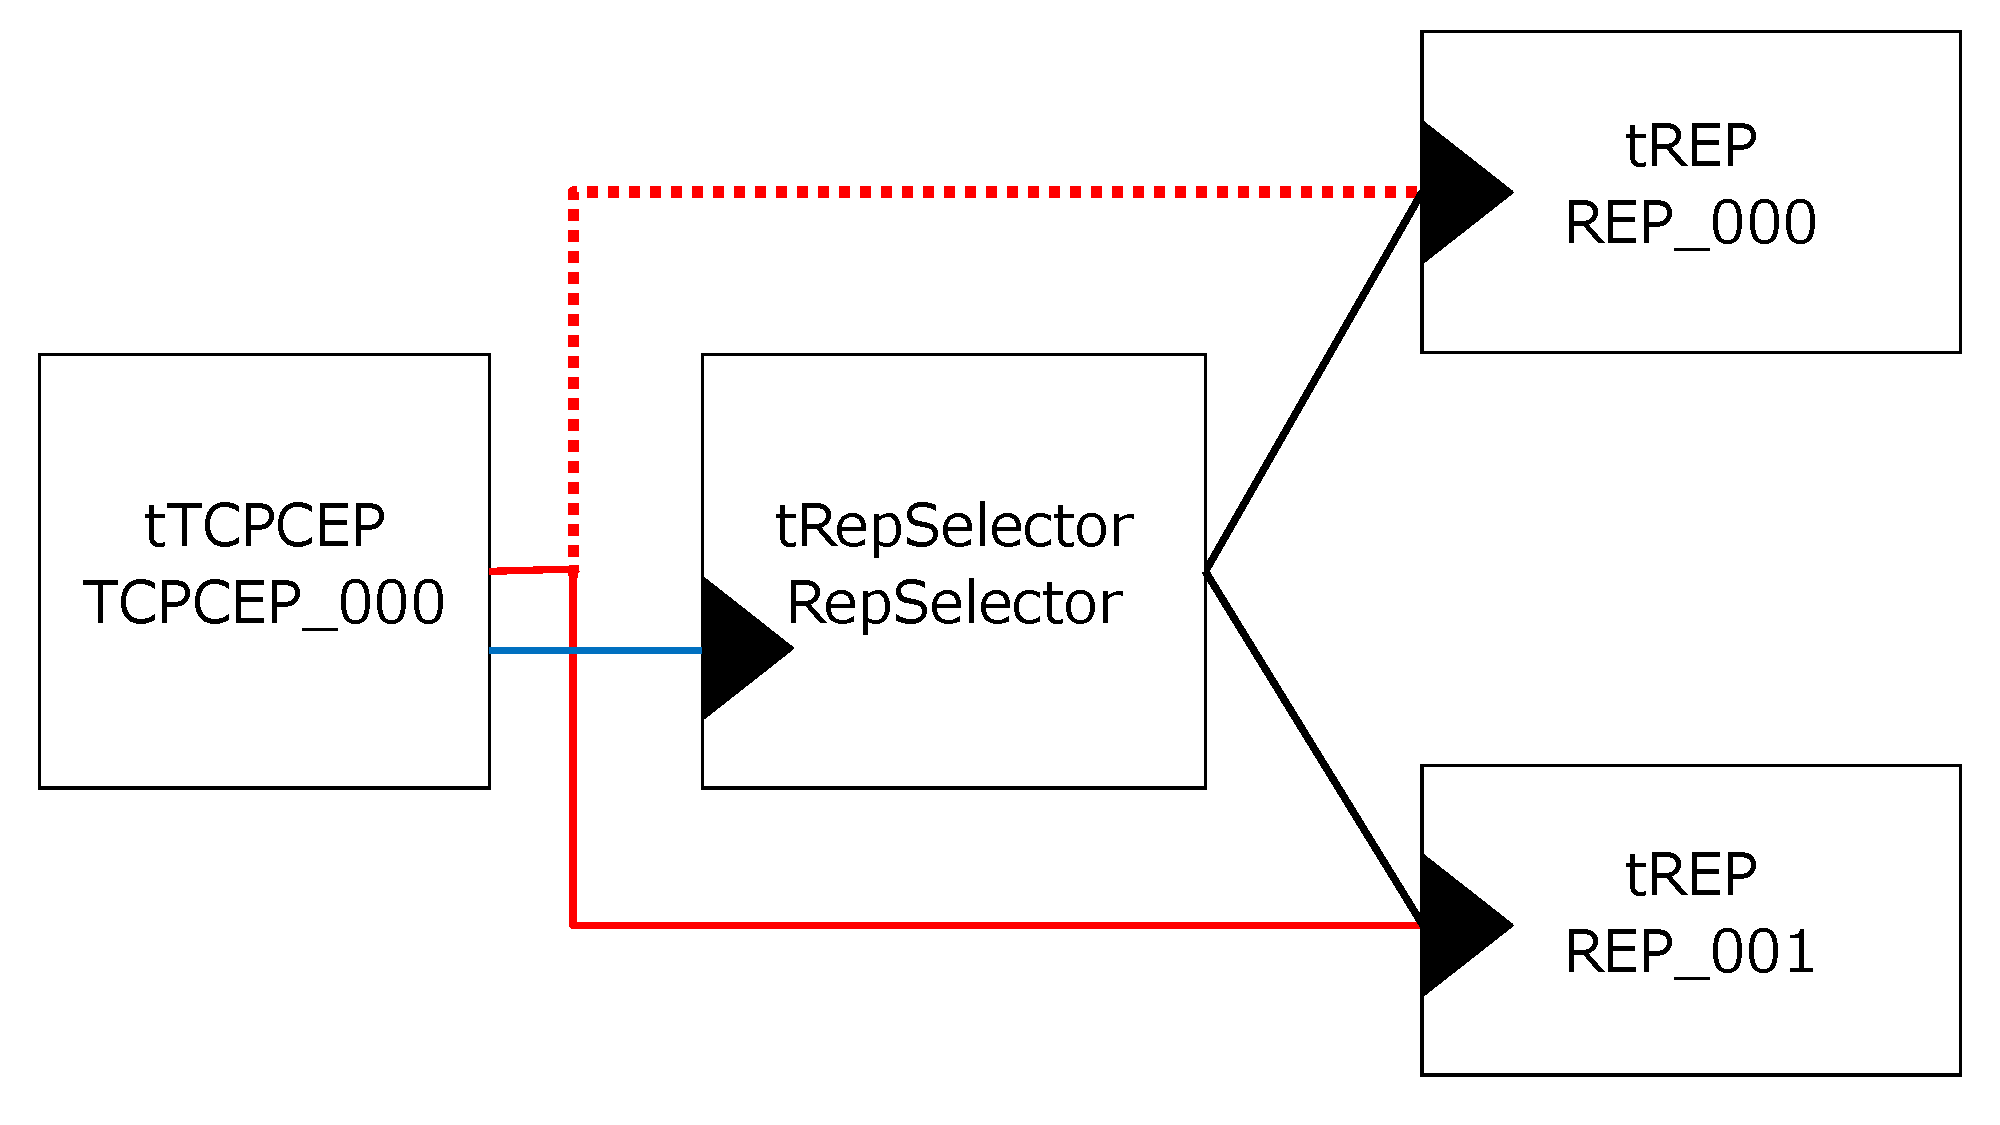
\includegraphics[width=7.0cm,clip]{figure/DynamicConnectionUseCase.pdf}
    \caption{Dynamic connection between CEP and REP}
    \label{fig:DynamicConnectionUseCase}
\end{figure}

To utilize dynamic connection, the selector should be defined.
The selector connects all the components that can be dynamically connnected, to refer the descripter of them.
Descriptor is an identifier to access the component.
cREP ports are call ports array, which connect the number of tREP cells (Line 9 in Fig. \ref{src:DynamicCDLcode}).
{\it [ref\_desc]} is described to identify the call port refers to descriptors. 
In the case of Fig. \ref{fig:DynamicConnectionUseCase}, the tRepSelector cell connects all tREP cells.

A CEP component has two call ports.
cRepSelector port connects eRepSelector port of tRepSelector cell and cREP4 port connects either of tREP cells (Lines 13-15 in Fig. \ref{src:DynamicCDLcode}).
cREP port is defined with {\it [dynamic]} to identify the call port dynamically switch the components.
The call port with {\it [dynamic]} specifier is not optimized and allocated in RAM by a plug-in.

\begin{figure}[t]
\centering
\begin{lstlisting}
signature sRepSelector {
    void  getRep([out]Descriptor(sREP4) *desc,
                 [in]int_t i);
};

celltype tRepSelector {
    entry sRepSelector eRepSelector;
    [ref_desc]
        call sREP4 cREP[NUM_REP];
};

celltype tTCPCEP {
    call sRepSelector cRepSelector;
    [dynamic]
        call sREP4 cREP;
    /* Omit: other call/entry ports */
    /* Omit: attributes and variables */
};
\end{lstlisting}
\caption{Signature and celltype description for dynamic connection}
\label{src:DynamicCDLcode}
\end{figure}

Fig. \ref{src:DynamicCcode} shows a sample code of dynamic connection.
The eAPI\_accept function is the function wrapping {\it tcp\_acp\_cep} with TECS, which is utilized to be the state waiting for connection request.
In the function, dynamic connection is performed as shown in Fig. \ref{src:DynamicCcode}.
First, get the descriptor of REP to be joined (Line 3 in Fig. \ref{src:DynamicCcode}).
The first argument, {\it \&desc}, is a variable to store the descriptor information, and the second argument, {\it repid}, is the index of tREP cells.
Next, set the desctriptor (Line 5 in Fig. \ref{src:DynamicCcode}).
cREP port combines the tREP cell that descriptor specify.
Thus, the tCEP cell can call the function of tREP cell to be joined (Line 7 in Fig. \ref{src:DynamicCcode}).

\begin{figure}[t]
\centering
\begin{lstlisting}
eAPI_accept (.., ..) {
    /* Get a descripter of intended REP cell */
    cRepSelector_getRep(&desc, repid);
    /* Set the descripter */
    cREP_set_descriptor(desc);
    /* Call the function of intended REP cell */
    cREP_getEndpoint();
}
\end{lstlisting}
\caption{Accept function (a dynamic connection example)}
\label{src:DynamicCcode}
\end{figure}

\subsection{TECS Adapter}
\label{sec:TECS Adapter}

TECS supports {\it Adapter} functionality which enables to call a function in TECS from existing C codes.
An adapter connects a TECS component, and links a C function to a TECS function shown as Fig. \ref{fig:TECS_Adapter}.
Software developers can utilize an existing application for TECS owing to the adapter.

\begin{figure}[t]
    \centering
    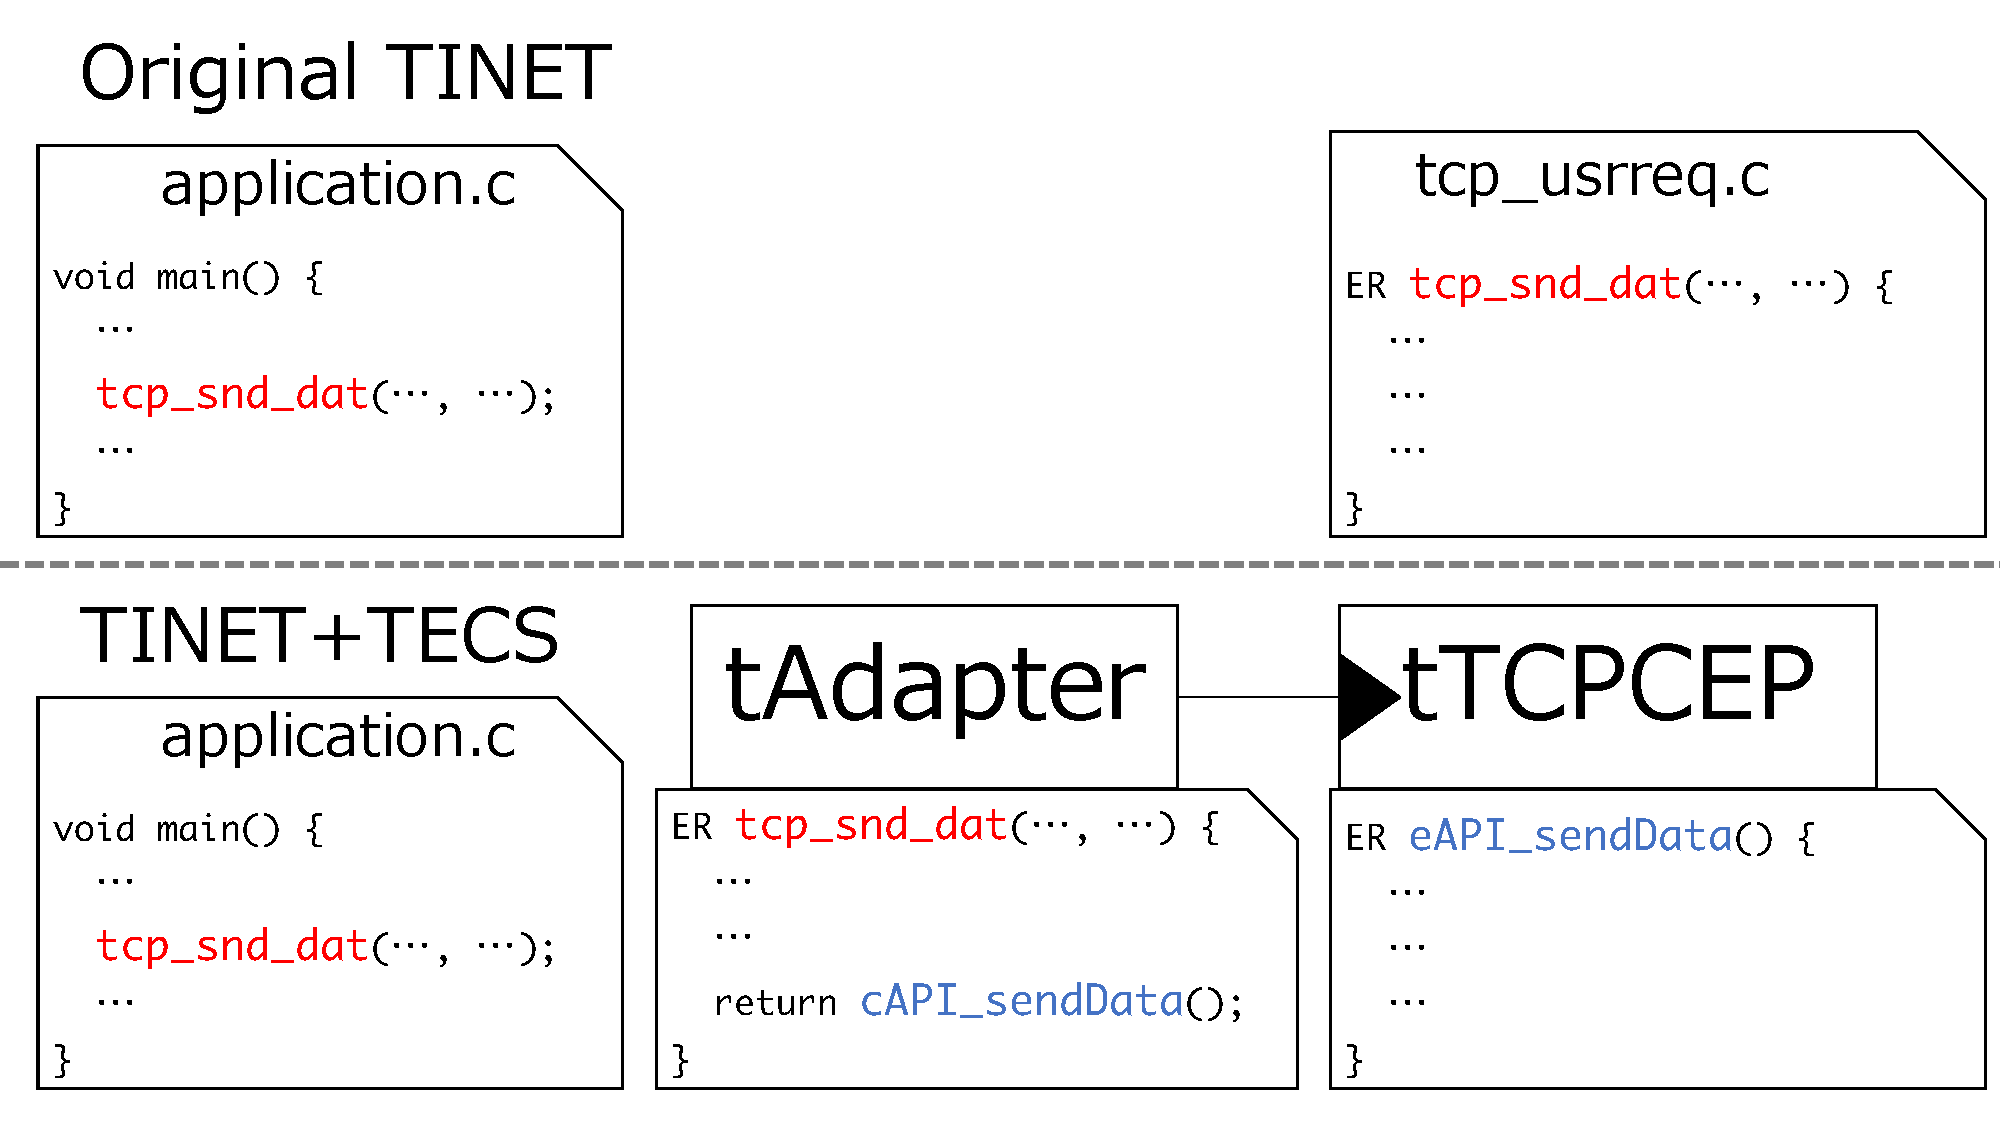
\includegraphics[width=7.0cm,clip]{figure/TECS_Adapter.pdf}
    \caption{TECS Adapter}
    \label{fig:TECS_Adapter}
\end{figure}

\section{Evaluation}
\label{sec:Evaluation}

\subsection{Evaluation environment}

GR-PEACH is employed as the evaluation board.
We connected the board and the host PC with a LAN cable, and evaluated the data transmission and reception.
The detail specification of the board is shown in TABLE \ref{tab:EvaluationBoardEnvironment}.
We also employ TINET 1.5.4 and the compiler arm-none-eabi--gcc 5.2.

\begin{table}[t]
    \centering
    \caption{Evaluation Board Environment}
    \begin{tabular}{l|l}
        \hline\hline
        Board           &   GR-PEACH                \\
        CPU             &   Cortex-A9 RZ/A1H 400MHz \\
        Flash ROM       &   8 MB                    \\
        RAM             &   10 MB                   \\
        LAN Controller  &   LAN8710A                \\
        \hline
    \end{tabular}
    \label{tab:EvaluationBoardEnvironment}
\end{table}


\section{Related Work}
\label{sec:Related Work}

Open-source TCP/IP protocol stacks for embedded systems have been developed such uIP \cite{par:uIP}, lwIP \cite{par:lwIP}.

{\bf uIP:}
uIP (microIP) is a very small TCP/IP stack intended for tiny 8-bit and 16-bit microcontrollers.
uIP only requires about five kilobytes of code size and several hundred bytes of RAM.
uIP has been ported to various systems and has found its way into many commercial products.
After ver. 1.0 is released, later versions of uIP, including uIPv6, are integrated with Contiki OS \cite{par:Contiki},\cite{url:Contiki}, an operating system to connect tiny microcontroller to the Internet.

{\bf lwIP:}
lwIP (lightweightIP) is a small TCP/IP implementation for embedded systems.
The focus of lwIP is to reduce memory resource while still having a full scale TCP.
lwIP requires about 40 kilobytes of ROM and tens of kilobytes of RAM.
lwIP is larger than uIP, but provides better throughput.

{\bf CiAO/IP:}


\section{Conclusion}
\label{sec:Conclusion}

In the future, the proposed framework will cooperate with mruby on TECS \cite{par:mrubyonTECS}.
Note that mruby is a scripting language for embedded systems \cite{par:mruby}.
We will support the functionality that TINET functions can be utilized from mruby programs as an extension of mruby-socket \cite{url:mruby-library}.

    
% conference papers do not normally have an appendix


% use section* for acknowledgment
\section*{Acknowledgment}

The authers would like to thank Hiroaki Nagashima for supporting this research.
This work is supported by JSPS KAKENHI Grant Number 15H05305.

% trigger a \newpage just before the given reference
% number - used to balance the columns on the last page
% adjust value as needed - may need to be readjusted if
% the document is modified later
%\IEEEtriggeratref{8}
% The "triggered" command can be changed if desired:
%\IEEEtriggercmd{\enlargethispage{-5in}}

% references section
\bibliographystyle{IEEEtranBST2/IEEEtran}
\bibliography{ref}

% that's all folks
\end{document}
